
%(BEGIN_QUESTION)
% Copyright 2015, Tony R. Kuphaldt, released under the Creative Commons Attribution License (v 1.0)
% This means you may do almost anything with this work of mine, so long as you give me proper credit

Suppose the solenoid energizes when the pushbutton switch is pressed and de-energizes when the pushbutton is released just as it is supposed to, but the lamp never energizes regardless of the pushbutton switch's state:

$$\includegraphics[width=15.5cm]{i03136x01.eps}$$

Identify the likelihood of each specified fault for this circuit.  Consider each fault one at a time (i.e. no coincidental faults), determining whether or not each fault could independently account for {\it all} measurements and symptoms in this circuit.

% No blank lines allowed between lines of an \halign structure!
% I use comments (%) instead, so that TeX doesn't choke.

$$\vbox{\offinterlineskip
\halign{\strut
\vrule \quad\hfil # \ \hfil & 
\vrule \quad\hfil # \ \hfil & 
\vrule \quad\hfil # \ \hfil \vrule \cr
\noalign{\hrule}
%
% First row
{\bf Fault} & {\bf Possible} & {\bf Impossible} \cr
%
\noalign{\hrule}
%
% Another row
Pushbutton switch failed open &  &  \cr
%
\noalign{\hrule}
%
% Another row
NC relay contact failed open &  &  \cr
%
\noalign{\hrule}
%
% Another row
NO relay contact failed open &  &  \cr
%
\noalign{\hrule}
%
% Another row
Relay coil failed open &  &  \cr
%
\noalign{\hrule}
%
% Another row
480 volt fuse(s) blown &  &  \cr
%
\noalign{\hrule}
%
% Another row
Pushbutton switch failed shorted &  &  \cr
%
\noalign{\hrule}
%
% Another row
NC relay contact failed shorted &  &  \cr
%
\noalign{\hrule}
%
% Another row
NO relay contact failed shorted &  &  \cr
%
\noalign{\hrule}
%
% Another row
Relay coil failed shorted &  &  \cr
%
\noalign{\hrule}
%
% Another row
24 VDC source dead &  &  \cr
%
\noalign{\hrule}
} % End of \halign 
}$$ % End of \vbox


\vfil 

\underbar{file i03136}
\eject
%(END_QUESTION)





%(BEGIN_ANSWER)

This is a graded question -- no answers or hints given!

%(END_ANSWER)





%(BEGIN_NOTES)

The fact that the solenoid behaves exactly as it should tells us the relay coil circuit is fully functioning, as is the AC circuit from source to solenoid.  The only suspect portion is that which controls the lamp.

% No blank lines allowed between lines of an \halign structure!
% I use comments (%) instead, so that TeX doesn't choke.

$$\vbox{\offinterlineskip
\halign{\strut
\vrule \quad\hfil # \ \hfil & 
\vrule \quad\hfil # \ \hfil & 
\vrule \quad\hfil # \ \hfil \vrule \cr
\noalign{\hrule}
%
% First row
{\bf Fault} & {\bf Possible} & {\bf Impossible} \cr
%
\noalign{\hrule}
%
% Another row
Pushbutton switch failed open &  & $\surd$ \cr
%
\noalign{\hrule}
%
% Another row
NC relay contact failed open &  & $\surd$ \cr
%
\noalign{\hrule}
%
% Another row
NO relay contact failed open & $\surd$ &  \cr
%
\noalign{\hrule}
%
% Another row
Relay coil failed open &  & $\surd$ \cr
%
\noalign{\hrule}
%
% Another row
480 volt fuse(s) blown &  & $\surd$ \cr
%
\noalign{\hrule}
%
% Another row
Pushbutton switch failed shorted &  & $\surd$ \cr
%
\noalign{\hrule}
%
% Another row
NC relay contact failed shorted &  & $\surd$ \cr
%
\noalign{\hrule}
%
% Another row
NO relay contact failed shorted &  & $\surd$ \cr
%
\noalign{\hrule}
%
% Another row
Relay coil failed shorted &  & $\surd$ \cr
%
\noalign{\hrule}
%
% Another row
24 VDC source dead &  & $\surd$ \cr
%
\noalign{\hrule}
} % End of \halign 
}$$ % End of \vbox

A fault not listed in this table is that of the lamp being failed open.

%INDEX% Troubleshooting review: electric circuits

%(END_NOTES)


